\documentclass{article}
\usepackage{xunicode}
\usepackage{fontspec}
\usepackage[frenchb]{babel}
\usepackage{graphicx}
\usepackage{listings}
\usepackage[T1]{fontenc}
\usepackage{kpfonts}
\usepackage{amsmath}


\renewcommand*{\familydefault}{\sfdefault}

\renewcommand{\nobreakspace}{\nobreak\ }



\title{SUAPS}
\author{Clotilde \textsc{Massot} \and Alexandre \textsc{Garnier} \and Chimène Gaby \textsc{Nya Ngaha} \and Julien \textsc{Durillon}}

\begin{document}

\maketitle

\section{Analyse}

	\subsection{Utilisateurs}
		La population des utilisateurs du point de vue du logiciel est
		sensiblement homogène: ce sont des utilisateurs de terminal android.
		Leur but est de se renseigner sur et de s'inscrire aux sports.

		Aucune connaissance du domaine n'est vraiment requise pour utiliser
		l'application.

	\subsection{Tâches}
	
\section{Conception de l'interface}

	Une fois définie la population des utilisateurs cible, vient la définition et la conception d'une interface efficace. Ici l'efficacité consiste en une solution à même d'offrir les fonctions attendues des utilisateurs dans une interface adaptée à leur connaissance de l'environnement applicatif.

	\subsection{Concept d'interaction}
	
	En celà, il s'agit ici de parvenir à proposer une solution simple et claire à utiliser, de telle sorte que l'accession aux fonctions clés de l'application soient accessibles rapidement et intuitivement.
	
	Dès lors, et afin de proposer une interface potentiellement connue de l'utilisateur, nous avons eu pour idée de s'inspirer de l'application AlloCiné pour Android. Notamment l'analogie entre la recherche et l'affichage de films d'un côté, de sports d'un autre, s'est imposée d'elle-même.
	
	\begin{figure}[ht]
		\centering
		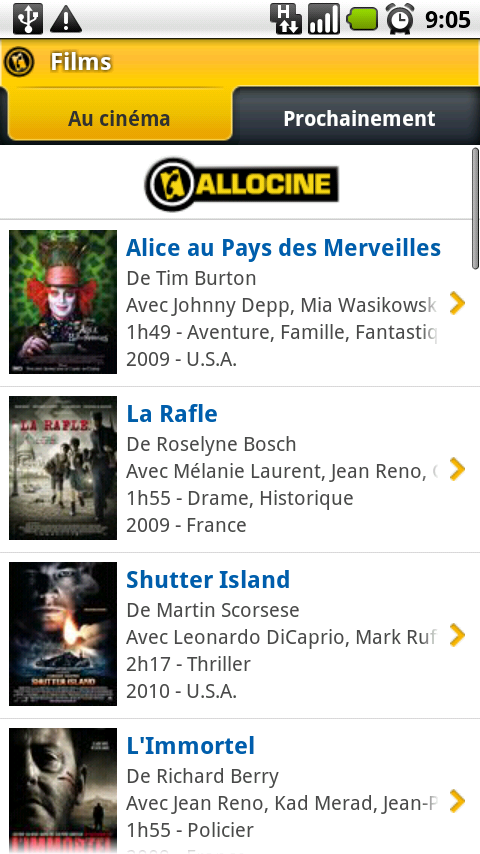
\includegraphics[width=0.5\textwidth]{allocine.png}
		\caption{Application AlloCiné : liste de films.}
		\label{fig:allocine}
	\end{figure}
	
	En outre, reprendre ainsi une interface que connaît l'utilisateur offre l'avantage de répondre à ses habitudes, automatisme	et exigences.
	
	\subsection{Écrans-clés}
	
	
	
	\subsection{Look and feel}
	
	
	
	\subsection{Prototypage}

	 Les tâches que l'utilisateur effectuera sont:

	    \paragraph{Parcours des sports}

	        Les sports sont classés par catégorie. Si on connaît le sport
	        cherché, l'accès à sa fiche se fait donc en 2 ou 3 \og clics\fg{}
	        maximum.

        \paragraph{Recherche de sport par critères}

            Pour un utilisateur cherchant à faire du sport en fonction de son
            emploi du temps: il pourra : rechercher par horaires, rechercher par
            lieu (contrainte géographique).

        \paragraph{Informations pratiques}

            Il est aussi possible de parcourir les lieux et d'en obtenir
            l'adresse ou le numéro.

        \paragraph{Inscription}

            La possibilité de s'inscrire à un sport peut aussi être proposée: il
            faut cependant passer par l'authentification inhérente à
            l'université.


    \subsection{Scénarii d'utilisation}

    Étant donné qu'il n'y a qu'une seule classe d'utilisateur, nous ne
    préciserons pas la classe effectuant chaque scénario.

        \paragraph{Accès à un sport}

            Dans ce cas, l'utilisateur lance l'application, choisit l'onglet
            Activités, choisit la catégorie voulue, puis sélectionne le sport.

            Il peut ensuite accéder à la fiche du lieu ou se déroule le sport, ou s'inscrire.

        \paragraph{Prospection par lieu}

            Dans ce scénario, l'utilisateur cherche un sport se déroulant dans un
            certain lieu. Il recherche donc dans la liste les lieux celui qui
            l'intéresse (on peut utiliser ici la géolocalisation pour avoir le
            lieu le plus proche). Une fois sur la fiche descriptive d'un lieu,
            on peut accéder aux sports qui s'y déroulent.

        \paragraph{Recherche par horaire}

            L'utilisateur va dans l'onglet \og Horaires\fg{} et entre ses vœux
            en terme de disponibilité. Les sports qui sont disponibles s'affichent.


\end{document}

